\documentclass[12pt,letterpaper]{article}
\usepackage[margin=1.0in]{geometry}
\usepackage[utf8]{inputenc}
\usepackage{cite}
\usepackage{amsmath}
\usepackage{amsfonts}
\usepackage{amssymb}
\usepackage{makeidx}
\usepackage{graphicx}
\usepackage{hyperref}
\setlength\parindent{0pt}
\usepackage[framed,numbered,autolinebreaks,useliterate]{mcode}

\author{STUDENT NAME}
\title{Lab9: Force measurement using a load cell and MatLab.}

\begin{document}

\maketitle

\section{Objectives}

This lab exercise aims to gain hands-on experience in using a load cell and signal conditioning to measure forces. In addition, the student will learn how to make a simple Graphical User Interface (GUI) in MatLab.

\section{Introduction}
Force and Torque measurement are important indicators of stress in stationary structures as well as power in machinery. The most common methods of force measurement are load cells. Load cells use strain gages to convert stress into strain, and subsequently strain into electric signals. In this lab you will learn how to calibrate a load cell using various weights and how to read the output from the load cell into a computer. Figure \ref{fig:Lab9_S-typeLoadCell} shows an example of an S-type load cell.\\

\begin{figure}
\centering
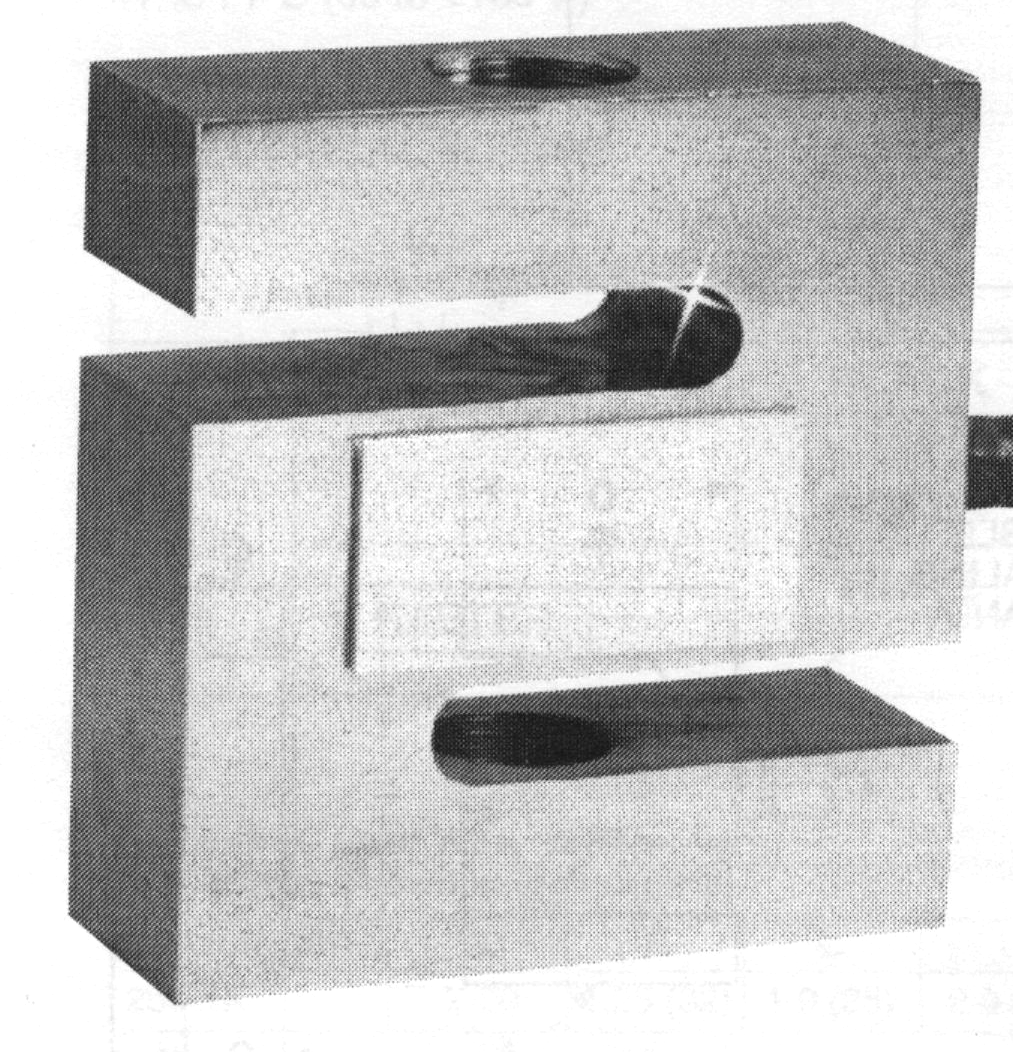
\includegraphics[width=.5\linewidth]{Lab9_S-typeLoadCell}
\caption{S-type load cell.}
\label{fig:Lab9_S-typeLoadCell}
\end{figure}

The cord lengths of the load cells are quite long, but DO NOT CUT THEM. If in practice you ever have to cut them, the calibration document is voided, and you will have to recalibrate the unit using known weights. Load cells always come with a calibration document, an example is given in Figure \ref{fig:Lab9_ForceMeasurementUsingLoadCell_CalibrationSheet}. Notice that the manufacturer used only three calibration points: 0 – 50 – 100 – 50 – 0 lbs.  The maximum output of the load cell is 30.032 milli-Volt at 100 lbs. This value is too small to be read into a computer directly. Therefore, an amplifier is needed to bring the voltage into a reasonable range that can be read by an analog input computer card such as -10 to 10 Volt. In the lab, we will use the TMO2 Load cell amplifier/conditioner module as shown in Figure \ref{fig:Lab9_LoadCellAmplifier}. This high quality amplifier allows calibration of the load cell and it contains a low pass filter to eliminate noise. Notice also that the calibration was performed using equipment that is traceable to the National Institute of Standards and Technology (NIST).\\

In the lab we will use a 50 lbs load cell with an 18 lbs load (a 24 pack of Coke Zero, as if that mattered). To bring the output of the Load Cell into a reasonable range, you need to choose a voltage range. In our case, it makes sense to have 50 lbs be represented by 10 V, which is the maximum output of the amplifier. This can be achieved by adjusting the GAIN screw on the TMO-2 module. However, it is also important that when no load is applied, the output is zero. In general amplifiers always have a zero (here BALANCE) and span (here GAIN) adjustment. The easiest method is to eliminate any bias first by adjusting the BALANCE such that the voltage output is zero. Then you adjust the GAIN when a known load is applied. After this, you need to iterate the BALANCE/GAIN adjustments since there are always some cross effects.\\ 

\begin{figure}
\centering
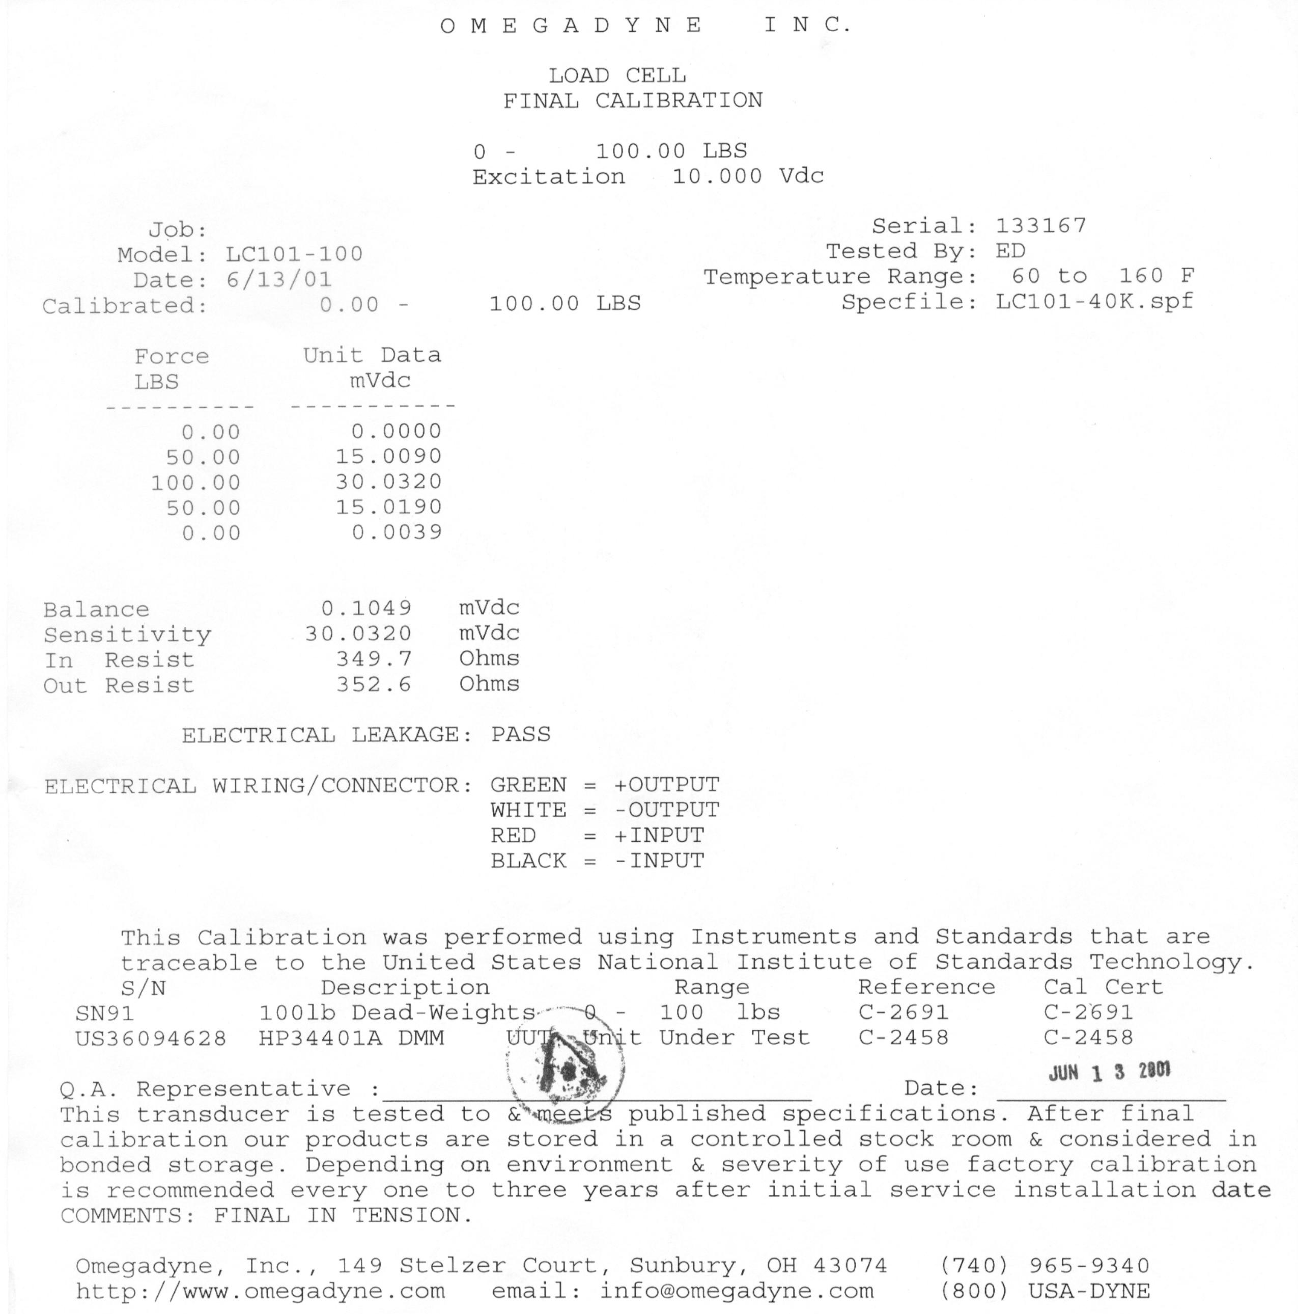
\includegraphics[width=1\linewidth]{Lab9_ForceMeasurementUsingLoadCell_CalibrationSheet}
\caption{Example calibration document of a LC101-100 Load Cell}
\label{fig:Lab9_ForceMeasurementUsingLoadCell_CalibrationSheet}
\end{figure}

\begin{figure}
\centering
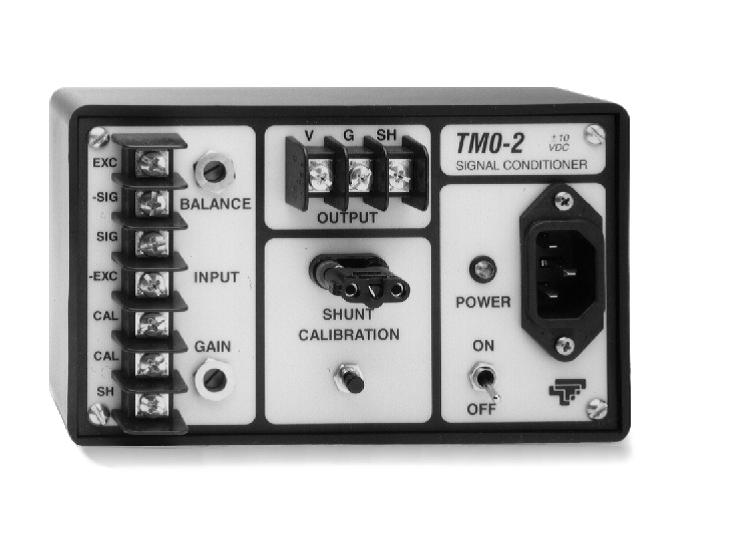
\includegraphics[width=0.6\linewidth]{Lab9_LoadCellAmplifier}
\caption{TMO load cell amplifier.}
\label{fig:Lab9_LoadCellAmplifier}
\end{figure}

In this lab we will use MatLab as our data acquisition program. MatLab can communicate with a NI6009 Data Acquisition module if the LabVIEW drivers are installed properly. To date, there is one problem with this configuration. Typically in MatLab one can set parameters (this is how Object Oriented programs work, you have an object and you can set its methods (these are procedures) and its properties, which are typically values. The current MatLab version (2014b) does not allow this (MatLab acknowledges this) so we need a work around. To set all inputs to Single Ended, we need to ground all complementary inputs of the Analog Input lines. Since we are using Analog Input 0 (AI0), we need to ground Analog Input 4 (which is the pin right next to AI0). 

The software in this lab will be written in MatLab using a Graphical User Interface. First, we will build a GIU by typing "guide" in the command prompt, see Figure \ref{fig:Lab9_LoadCellMeasurementGUIDE}. This program allows you to put controls (such a sliders, buttons, axes (for graphical output or images), text boxes etc.) on the background. For the data acquisition program we are going to have one axes (to put in an image of a load cell), three Static Text output (one for the measured value in Volt, one for the force in lbs, and one for the force in Newton), as well as a slider (which indicates the force in Newtons in a graphical way). We will add a button to Stop the program. The complete GUI looks as shown in Figure \ref{fig:Lab9_LoadCellMeasurementGUI}.

\begin{figure}
\centering
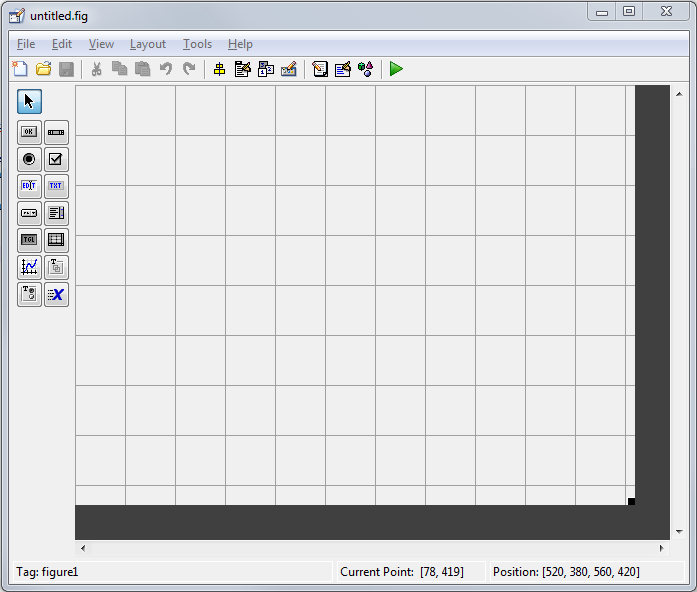
\includegraphics[width=0.8\linewidth]{Lab9_LoadCellMeasurementGUIDE}
\caption{MatLab program to build Graphical User Interfaces (GUIs)}
\label{fig:Lab9_LoadCellMeasurementGUIDE}
\end{figure}

Every object in your GUI has properties, double click on them and firstly, change the Tag to something logical. For instance, the Tag value of the picture axis call it "LoadCellPictureAxis". The Tag of the top Static Text box should show the load cell output in volt, so call it "LoadCellOutputVolt". The slider Tag, call it "LoadCellOutputSlider". You get the idea.

\begin{figure}
\centering
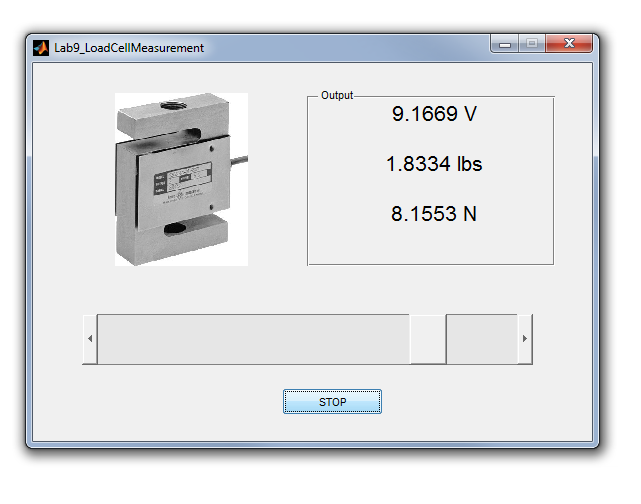
\includegraphics[width=0.6\linewidth]{Lab9_LoadCellMeasurementGUI}
\caption{Lab9: Load cell measurement: MatLab Graphical User Interface}
\label{fig:Lab9_LoadCellMeasurementGUI}
\end{figure}

When you are finished with the GUI you save the program, and it automatically generates a file with the same name but with extension ".m". There is a lot in this file that does not pertain to you, you'll have to learn to live with that. However, after the following lines, you can enter your main program. 

\begin{lstlisting}
% UIWAIT makes Lab9_LoadCellMeasurement wait for user response (see UIRESUME)
% uiwait(handles.figure1);
\end{lstlisting}

\newpage
Here are code snippets that you need to complete the program. First we need to put the picture in the axis (note that my name for the axis is LoadCellPictureAxis). The variable YN is related to the Stop button, which has its own function (this is what event driven coding is all about, every event triggers a function to be executed). Since we are using the YN variable here as well as in the Stop button function, it needs to be global.

\begin{lstlisting}
% UIWAIT makes Lab9_LoadCellMeasurement wait for user response (see UIRESUME)
% uiwait(handles.figure1);

% =========== Start user code =============================================
global YN
clc

% Put image in the top left axes
StartImage        =  imread('LoadCellImage.jpg');
set(handles.LoadCellPictureAxis,'HandleVisibility','ON');
axes(handles.LoadCellPictureAxis);
image(StartImage);
axis equal;
axis tight;
axis off;
\end{lstlisting}

We need a few constant values. We have a 50 lbs load cell and we want to use the full range of the 6008 (10 Volt) so the Lbs2Volt value = 10/50. We also need a conversion value from lbs to Newton which can be found on the internet:


\begin{lstlisting}
%=============================== Constants ===============================
Lbs2Volt = 10/50; % (We are using a 50 lbs Load Cell, at 10 Volt input
Lbs2N    = 4.44822162825;
\end{lstlisting}

Next we need to create a session in Matlab to do data acquisition (we only use and analog input with a single input terminal being AI0). The code shows that the commented line setting the input to "SingleEnded" does not work (this is a known problem with MatLab), so you need to hardwire Analog input 4 (AI4) to ground.

\begin{lstlisting}
%================= Session Based NI functionality (Windows 7) =======
daq.getDevices;
s                 = daq.createSession('ni');

% ========================== Setup Input ========================
Ch_input          = s.addAnalogInputChannel('Dev1',[0],'Voltage')
%set(Ch_input,'TerminalConfig','SingleEnded') % This does not work (MatLab acknowledges)!
\end{lstlisting}

Now we need the main program: We make a while loop and keep repeating as long as the YN variable is 0 (meaning the Stop button is not pressed). As soon as the Stop button does get pressed, the global YN variable becomes '1' and the program drops out of the loop.\\

Data continuously gets values from the 6008 board, in Volt. This is translated into the Load in lbs (using the Lbs2Volt) variable, and to the Load in Newton using the Lbs2N variable. Now we need to write these values to the Static Text boxes (I called them LoadCellOutputVolt, LoadCellOutputLbs and LoadCellOutputNewton), check if this is what you called them. To write a string to the object, you use the set function as shown. The "handles" variable is used internally by MatLab to store all handles to all object, don't fret over that thing.\\

Now we need to write a value to the slider which graphically indicates the load level in Lbs. Make sure that you set the min and max value of the slider (I called it LoadCellOutputSlider) to +50 and -50 (since we have a 50 lbs load cell, which can be in compression or tension). Also see how we catch potential errors, if you write a value to the slider outside its limits you'll get an error message. To prevent that you first read the min and max values (check where that happens) and then you only write values if they are within the proper range, otherwise you write a zero to set the slider in the center. The pause command is used to give the program time to update the text boxes and the slider.

%\newpage
\begin{lstlisting}
YN = 0;
while YN == 0
   Data              = s.inputSingleScan;                        % Volt
   Load_lbs          = Data/Lbs2Volt;
   Load_N            = Load_lbs* Lbs2N;
   
   set(handles.LoadCellOutputVolt,'String',[num2str(Data) ' V']);
   set(handles.LoadCellOutputLbs,'String',[num2str(Load_lbs) ' lbs']);
   set(handles.LoadCellOutputNewton,'String',[num2str(Load_N) ' N']);
   
   LoadSliderMax     = get(handles.LoadCellOutputSlider,'Max');
   LoadSliderMin     = get(handles.LoadCellOutputSlider,'Min');
   
   if Load_lbs < LoadSliderMax && Load_lbs > LoadSliderMin
      set(handles.LoadCellOutputSlider,'Value',Load_lbs);
   else
      set(handles.LoadCellOutputSlider,'Value',0);
   end
   pause(0.1)
end
\end{lstlisting}


Finally, we need to catch the value of the Stop button. When it gets pressed the function as shown is executed, and we use that to get the value of the Stop button (which is binary it is either 0 (not pressed) or 1 (pressed) .

\begin{lstlisting}
% --- Executes on button press in StopButton.
function StopButton_Callback(hObject, eventdata, handles)
global YN
% hObject    handle to StopButton (see GCBO)
% eventdata  reserved - to be defined in a future version of MATLAB
% handles    structure with handles and user data (see GUIDATA)
YN                = get(handles.StopButton,'Value')
\end{lstlisting}


\section{Equipment}

\begin{enumerate}
\item Power supply
\item Computer with MatLab® and Data Acquisition Toolbox
\item USB 6008 DAQ Module
\item DMM
\item Omega LC101-100 S-type Load Cell 
\item Breadboard and signal conditioning components
\item TMO2 Load cell amplifier/conditioner module.
\end{enumerate}

\section{Procedures}	 
\begin{enumerate}
\item Download the specifications of the LC101-100 (100 lbs) load cell \href{http://abe-research.illinois.edu/Faculty/grift/ABE425_2015/Specs/LC101.pdf}{here}. 
\item Download AND READ the \href{http://abe-research.illinois.edu/Faculty/grift/ABE425_2015/Specs/tmo2.pdf}{Operator Manual} of the TMO-2 Load cell amplifier / conditioner.
\item Connect the load cell to the Load Cell Amplifier using the Operator Manual. 
\item Build the Graphical User Interface.
\item Once you have a working program, you need to hook up the output of the load cell amplifier (Figure \ref{fig:Lab9_LoadCellAmplifier}) to that AI0 of the 6008 (V is positive G goes to ground). Now you calibrate your complete system by first measuring the output without a load and turning the Balance adjustment to zero (don't hook up a voltmeter your program shows that voltage). Secondly, your known load is 18 lbs (approx) which is 36 \% of the max load (50 lbs). Therefore with a load of 18 lbs you should read 3.6 Volt. Use the Gain adjustment to set that value. However, if you remove the load you'll see that the zero has drifted, so you need to readjust the Balance to set it back to zero. You may need to go back and forth between Balance and Gain a few times to get it just right.
\end{enumerate}


\section{Questions}

Q1:	Load cells typically consist of strain gages that are placed in a Wheatstone bridge configuration. Why is it necessary to use a bridge? \\
A1:\\

Q2:	What are common types of load cell forms, other than the S-type we used here?\\
A2:\\

\end{document}
